\documentclass[noauthor, nooutcomes]{ximera}

\input{../preamble}
\author{Kenneth Berglund}
\license{Creative Commons Attribution-ShareAlike 4.0 International License}
\acknowledgement{https://www.stitz-zeager.com/szca07042013.pdf}

\title{Solving Inequalities without a Graph}

%This is so the pictures show up
\pgfplotsset{compat=1.5.1}

%This is also for pictures
\usetikzlibrary{calc}

%This makes hyperbolas. I found it at https://newbedev.com/can-one-draw-a-hyperbola-with-arguments-in-tikz
%
% #1 optional parameters for \draw
% #2 angle of rotation in degrees
% #3 offset of center as (pointx, pointy) or (name-o-coordinate)
% #4 length of plus (semi)axis, that is axis which hyperbola crosses
% #5 length of minus (semi)axis
% #6 how much of hyperbola to draw in degrees, with 90 you’d reach infinity
%
\newcommand\tikzhyperbola[6][thick]{%
    \draw [#1, rotate around={#2: (0, 0)}, shift=#3]
        plot [variable = \t, samples=1000, domain=-#6:#6] ({#4 / cos( \t )}, {#5 * tan( \t )});
    \draw [#1, rotate around={#2: (0, 0)}, shift=#3]
        plot [variable = \t, samples=1000, domain=-#6:#6] ({-#4 / cos( \t )}, {#5 * tan( \t )});
}

\begin{document}
\begin{abstract}
  
\end{abstract}
\maketitle
\licenseSZ

\begin{motivatingQuestions}\begin{itemize}
	\item How can we find solutions to inequalities without using a graph?
	\item How can we use the zeros of functions to solve inequalities?
\end{itemize}\end{motivatingQuestions}

%\typeout{************************************************}
%\typeout{Introduction and the Importance of Zeros}
%\typeout{************************************************}
\section{Introduction and the Importance of Zeros}
In the previous section, we constructed the following graph to solve the inequality $f(x) \le 0$, where $f(x) = x^2 - x$.
\begin{image}
\begin{tikzpicture}
    \begin{axis}[xmin=-3, xmax=4]
         \addplot[domain=-2.2:3.2, <->]{x^2 - x} node{};
	\addplot[<->, dashed, very thick]{0} node{}; 
	\node (g) at (axis cs:2,6) {$y=f(x)$};
	\node (f) at (axis cs:-2,0.5) {$y=0$};
	\addplot[penColor, mark=*, only marks] coordinates {(0,0)};
	\addplot[penColor, mark=*, only marks] coordinates {(1,0)};
	\node(l) at (axis cs:-.5,-1) {$(0,0)$};
	\node(r) at (axis cs:1,-1) {$(1,0)$};
    \end{axis}
\end{tikzpicture}
\end{image}

We can see that the graph of $f$ does dip below the $x$-axis between its two $x$-intercepts.  The zeros of $f$ are $x=0$ and $x=1$ in this case and they divide the domain (the $x$-axis) into three intervals:  $(-\infty, 0)$, $(0, 1)$ and $(1, \infty)$.  For every number in $(-\infty, 0)$, the graph of $f$ is above the $x$-axis; in other words, $f(x) > 0$ for all $x$ in $(-\infty, 0)$. Similarly, $f(x) < 0$ for all $x$ in $(0,1)$, and $f(x) > 0$ for all $x$ in $(1, \infty)$.  We can schematically represent this with the \emph{sign diagram}\index{inequality ! sign diagram}\index{sign diagram ! for quadratic inequality} below.
\begin{image}
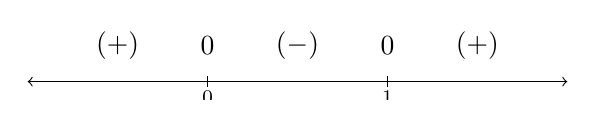
\begin{tikzpicture}
    \begin{axis}[axis equal image, ymin=-.1,ymax=.3,xmin=-1, xmax=2, axis x line=none, axis y line=none,]
	\draw[<->] (axis cs:-1, 0) -- (axis cs: 2, 0);
	\addplot[mark=|, only marks] coordinates {(0, 0)};
	\addplot[mark=|, only marks] coordinates {(1, 0)};
	\node[below] (z1) at (axis cs:0,0) {$\scriptstyle{0}$};	
	\node[below] (z2) at (axis cs:1,0) {$\scriptstyle{1}$};
	\node (a) at (axis cs:-0.5,0.2) {$(+)$};
	\node (b) at (axis cs:1.5,0.2) {$(+)$};
	\node (c) at (axis cs:0.5,0.2) {$(-)$};	
	\node (d) at (axis cs:0,0.2) {$0$};	
	\node (e) at (axis cs:1,0.2) {$0$};	
    \end{axis}
\end{tikzpicture}
\end{image}

Here, the $(+)$ above a portion of the number line indicates $f(x) > 0$ for those values of $x$; the $(-)$ indicates $f(x) < 0$ there.  The numbers labeled on the number line are the zeros of $f$, so we place $0$ above them.  We see at once that the solution to $f(x) < 0$ is $(0, 1)$. Adding in the zeros, the solution to $f(x) \le 0$ is $[0, 1]$. 

Our next goal is to establish a procedure by which we can generate the sign diagram without graphing the function.

%\typeout{************************************************}
%\typeout{Continuity and the Intermediate Value Theorem}
%\typeout{************************************************}
\section{Continuity and the Intermediate Value Theorem}
An important property of quadratic functions is that if the function is positive at one point and negative at another, the function must have at least one zero in between. Graphically, this means that a parabola can't be above the $x$-axis at one point and below the $x$-axis at another point without crossing the $x$-axis. 

This is a special case of a theorem called the Intermediate Value Theorem, or IVT for short. To talk about the IVT, we first need to discuss what it means for a function to be \emph{continuous}. 

\begin{definition}\emph{(Informal.)}
We say a function $f$ on an interval is \index{continuous}\dfn{continuous} if the graph of $f$ has no `breaks' or `holes' on that interval. 
\end{definition}

In further courses, you will learn a more formal definition of continuity, but for now, this will suffice.

\begin{example}
\begin{enumerate}
	\item Linear and quadratic functions are continuous.
	\item In fact, all of our famous functions are continuous where they are defined. 
	\item All polynomials are continuous.
	\item Rational functions are continuous where they are defined. In particular, $\frac{1}{x}$ is continuous on its domain, $(- \infty, 0) \cup (0, \infty)$. 
	\item If $f$ and $g$ are continuous functions, so are $f + g$ and $f \cdot g$. 
\end{enumerate}
\end{example}

\begin{image}
\begin{tikzpicture}
    \begin{axis}
        \addplot[smooth, <->, domain=-7:7]{abs(x)} node{};
    \end{axis}
\end{tikzpicture}
\hspace{10mm}
\begin{tikzpicture}
    \begin{axis}
	\addplot[mark=o, only marks] coordinates {(5,5)};
	\addplot[mark=*, only marks] coordinates {(5,3)};
        \draw (axis cs:0, 0) -- (axis cs: 4.9, 4.9);
	\draw[->] (axis cs:5.1, 5.1) -- (axis cs:7,7);
	\draw (axis cs:0, 0) -- (axis cs: -2.9, 2.9);
	\addplot[mark=o, only marks] coordinates {(-3,3)};
	\addplot[mark=*, only marks] coordinates {(-3,4)};
	\draw[<-] (axis cs:-7, 4) -- (axis cs: -3, 4);
    \end{axis}
\end{tikzpicture}
\end{image}
The function whose graph is shown on the left above is continuous, while the function whose graph is shown on the right above is not, since it has breaks in its graph.

One way to think about continuous functions is that they are the functions whose graphs you could draw on an infinite piece of paper without ever taking your pencil off the paper (except where they aren't defined). You will encounter and learn about continuous functions more in-depth in calculus, but for now, familiarity at this level will be enough.

Now that we know about continuous functions, we can state our version of the IVT. 

\begin{theorem}[Intermediate Value Theorem (Zero Version)]
Suppose $f$ is a continuous function on an interval containing $x = a$ and $x = b$ with $a < b$. If $f(a)$ and $f(b)$ have different signs, then $f$ has at least one zero between $x = a$ and $x = b$; that is, for at least one real number $c$ such that $a < c < b$, we have $f(c) = 0$.
\end{theorem}

Reinterpreted, this means that the graph of a continuous function can't be above the $x$-axis at one point and below the $x$-axis at another point without crossing the $x$-axis. 

%You might ask whether the IVT is true for \emph{all} functions, not just continuous ones. In fact, it is not, and we can look at one of our famous functions to show this. Our only non-continuous famous function is tangent. Looking graphically, we see that $\tan\left(\frac{\pi}{4}\right)$ is positive and $\tan\left(\frac{3\pi}{4}\right)$ is negative, but the graph of tangent does not cross the $x$-axis on the interval $\left[\frac{\pi}{4}, \frac{3\pi}{4}\right]$.
%	\begin{image}
%		\begin{tikzpicture}
%			\begin{axis}[
%		            xmin=-1.6,xmax=6.75,ymin=-5.5,ymax=5.5,
%		            axis lines=center,
%		            xtick={-1.57, 0, 1.57, 3.142, 4.71, 6.28},
%		            xticklabels={$-\pi/2$, $0$, $\pi/2$, $\pi$, $3\pi/2$, $2\pi$},
%		            ytick={-5,...,5},
%		            minor ytick=,minor xtick=,
%		            width=0.75\linewidth,
%		            height=0.75\linewidth,
%		            xlabel=$x$, ylabel=$x$,
%%			    clip=false,
%			    grid style={dashed, gray!40}
%		          ]        
%		          \addplot [very thick, penColor, samples=100,smooth, domain=(-1.56:1.56)] {tan(deg(x))};% node [pos=0.51, penColor2, right] {$t(x)$};
%		          \addplot [very thick, penColor, samples=100,smooth, domain=(1.58:4.7)] {tan(deg(x))};
%		          \addplot [very thick, penColor, samples=100,smooth, domain=(4.9:6.4)] {tan(deg(x))};
%		                	
%	\addplot[penColor,mark=*, only marks] coordinates {(0.79,1)};
%	\addplot[penColor,mark=*, only marks] coordinates {(2.36,-1)};
%	\node[right] (a) at (axis cs:0.79,1) {$\left(\frac{\pi}{4}, 1\right)$};
%	\node[right] (b) at (axis cs:2.36,-1.2) {$\left(\frac{3\pi}{4}, -1\right)$};
%		        \end{axis}
%		\end{tikzpicture}
%	\end{image}



Here's how we'll use the IVT to solve inequalities of the form $f(x) > 0$, where $f$ is a continuous function. If a given interval does not contain a zero of $f$, then by the IVT either all the function values on the interval are positive or they're all negative. In this way, the IVT allows us to determine the sign of \emph{all} of the function values on the interval by testing the function at just \emph{one} value in the interval, which we're free to choose. 

This gives us the following steps for solving an inequality involving a continuous function.

\begin{enumerate}

\item  Rewrite the inequality, if necessary, as a continuous function $f(x)$ on one side of the inequality and $0$ on the other.

\item  Find the zeros of $f$ and place them on the number line with the number $0$ above them.

\item  Choose a real number, called a \emph{test value}, in each of the intervals determined in step 2. 

\item  Determine the sign of $f(x)$ for each test value in step 3, and write that sign above the corresponding interval.

\item  Choose the intervals which correspond to the correct sign to solve the inequality.

\end{enumerate}

As you can see, the zeros of continuous functions are important, so in the examples that follow, we'll highlight the techniques we use to find zeros. It may also be useful to review methods for finding zeros that you've seen before.

%\typeout{************************************************}
%\typeout{Solving Inequalities Algebraically}
%\typeout{************************************************}
\section{Solving Inequalities Algebraically}
\begin{example}
Solve the inequality $3x^2 + x < 6x - 2$.
\end{example}
\begin{explanation}
To start, let's put the inequality in a nice form, with a continuous function on one side and 0 on the other. It doesn't matter which side the 0 is on, so we'll choose to rewrite the inequality as $3x^2 - 5x + 2 < 0$. Since quadratic functions are continuous, we can use the steps outlined in the previous section to solve the inequality.

First, we find the zeros of $f$, where $f(x) = 3x^2 - 5x + 2$. We could do this by using the quadratic formula, but let's factor. Factoring gives us $f(x) = (3x - 2)(x - 1)$. In order for $f(x) = 0$ to be true, we need $3x - 2 = 0$ or $x - 1 = 0$. This tells us that the zeros of $f$ are $x= \frac{2}{3}$ and $x = 1$. This gives us a good start to our sign diagram:

\begin{image}
\begin{tikzpicture}
    \begin{axis}[axis equal image, ymin=-.15,ymax=.3,xmin=-1, xmax=2, axis x line=none, axis y line=none,]
	\draw[<->] (axis cs:-1, 0) -- (axis cs: 2, 0);
	\addplot[mark=|, only marks] coordinates {(0, 0)};
	\addplot[mark=|, only marks] coordinates {(1, 0)};
	\node[below] (z1) at (axis cs:0,0) {$\scriptstyle{\frac{2}{3}}$};	
	\node[below] (z2) at (axis cs:1,0) {$\scriptstyle{1}$};
	\node (a) at (axis cs:-0.5,0.2) {$$};
	\node (b) at (axis cs:1.5,0.2) {$$};
	\node (c) at (axis cs:0.5,0.2) {$$};	
	\node (d) at (axis cs:0,0.2) {$0$};	
	\node (e) at (axis cs:1,0.2) {$0$};	
    \end{axis}
\end{tikzpicture}
\end{image}

This sign diagram tells us that we have to check three intervals: $\left(-\infty, \frac{2}{3}\right)$, $\left(\frac{2}{3}, 1\right)$, and $(1, \infty)$. However, thanks to the IVT, we only need to check one test value per interval. Be careful not to choose $x = \frac{2}{3}$ or $x = 1$ as your test values!

For the interval $\left(-\infty, \frac{2}{3}\right)$, we choose $x = 0$ to be our test value and see that $f(0) = 3(0)^2 - 5(0) + 2 = 2$, which is positive. 

For the interval $\left(\frac{2}{3}, 1\right)$, we choose $x = \frac{5}{6}$ to be our test value and see that $f(0) = 3\left(\frac{5}{6}\right)^2 - 5\left(\frac{5}{6}\right) + 2 = \frac{25}{12} - \frac{25}{6} + 2 = -\frac{1}{12}$, which is negative. 

For the interval $\left(1, \infty\right)$, we choose $x = 2$ to be our test value and see that $f(2) = 3(2)^2 - 5(2) + 2 = 4$, which is positive. 

We can now update our sign diagram to the following:
\begin{image}
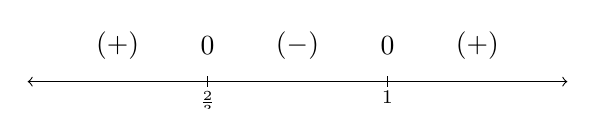
\begin{tikzpicture}
    \begin{axis}[axis equal image, ymin=-.15,ymax=.3,xmin=-1, xmax=2, axis x line=none, axis y line=none,]
	\draw[<->] (axis cs:-1, 0) -- (axis cs: 2, 0);
	\addplot[mark=|, only marks] coordinates {(0, 0)};
	\addplot[mark=|, only marks] coordinates {(1, 0)};
	\node[below] (z1) at (axis cs:0,0) {$\scriptstyle{\frac{2}{3}}$};	
	\node[below] (z2) at (axis cs:1,0) {$\scriptstyle{1}$};
	\node (a) at (axis cs:-0.5,0.2) {$(+)$};
	\node (b) at (axis cs:1.5,0.2) {$(+)$};
	\node (c) at (axis cs:0.5,0.2) {$(-)$};	
	\node (d) at (axis cs:0,0.2) {$0$};	
	\node (e) at (axis cs:1,0.2) {$0$};	
    \end{axis}
\end{tikzpicture}
\end{image}

Since we wanted to find where $f$ was negative, we choose $\left(\frac{2}{3}, 1\right)$ as the solution to the inequality.
\end{explanation}

\begin{example}
Solve the inequality $xe^x  \ge -x$.
\end{example}
\begin{explanation}
Rewriting our inequality, we have $xe^x + x \ge 0$. Since linear and exponential functions are continuous and products and sums of continuous functions are continuous, we know that the function $f$ defined by $f(x) = xe^x + x$ is a continuous function.

First, we find the zeros of $f$. We start by noticing that each term in $xe^x + x$ contains a factor of $x$, so we can factor that out and find $f(x) = x(e^x + 1)$. In order to solve the equation $f(x) = 0$, we need to solve $x = 0$ and $e^x + 1 = 0$. The first equation is already solved, and tells us that $x = 0$ is one zero of $f$. To solve the second equation, we calculate
\begin{align*}
e^x + 1 & = 0\\
e^x & = -1,
\end{align*}
and note that the exponential function is never negative, so there are no solutions. Therefore, the only zero of $f$ is $x = 0$. We now begin to construct the sign diagram.

\begin{image}
\begin{tikzpicture}
    \begin{axis}[axis equal image, ymin=-.1,ymax=.3,xmin=-1, xmax=1, axis y line=none,axis x line=none]
	\draw[<->] (axis cs:-1, 0) -- (axis cs: 1, 0);
	\addplot[mark=|, only marks] coordinates {(0, 0)};
	\node[below] (z1) at (axis cs:0,0) {$\scriptstyle{0}$};
	\node (a) at (axis cs:-0.5,0.2) {$$};
	\node (c) at (axis cs:0.5,0.2) {$$};	
	\node (d) at (axis cs:0,0.2) {$0$};
    \end{axis}
\end{tikzpicture}
\end{image}

This sign diagram tells us that we have to check two intervals: $\left(-\infty, 0\right)$ and $(0, \infty)$. Again, thanks to the IVT, we only need to check one test value per interval.

For the interval $\left(-\infty, 0\right)$, we choose $x = -1$ to be our test value and see that $f(-1) = e^{-1} - 1$, which is negative. To see that $e^{-1} - 1$ is negative, notice that $e^{-1} = \frac{1}{e}$, and since $e > 1$, $\frac{1}{e} < 1$. Therefore, when we subtract 1 from $e^{-1}$, we obtain a negative number. 

For the interval $\left(0, \infty\right)$, we choose $x = 1$ to be our test value and see that $f(1) = e^1 + 1$, which is positive.

We can now update our sign diagram to the following:
\begin{image}
\begin{tikzpicture}
    \begin{axis}[axis equal image, ymin=-.1,ymax=.3,xmin=-1, xmax=1, axis y line=none,axis x line=none]
	\draw[<->] (axis cs:-1, 0) -- (axis cs: 1, 0);
	\addplot[mark=|, only marks] coordinates {(0, 0)};
	\node[below] (z1) at (axis cs:0,0) {$\scriptstyle{0}$};
	\node (a) at (axis cs:-0.5,0.2) {$(-)$};
	\node (c) at (axis cs:0.5,0.2) {$(+)$};	
	\node (d) at (axis cs:0,0.2) {$0$};
    \end{axis}
\end{tikzpicture}
\end{image}

Since we wanted to find where $f$ was non-negative, we choose $[0, \infty)$ as the solution to the inequality. Remember to include 0 in the interval, since zeros of $f$ are also points where $f$ is non-negative.
\end{explanation}

\begin{example}
Solve the inequality $2^{x^2 - 3x} \ge 16$.
\end{example}
\begin{explanation}
We set $r(x) = 2^{x^2-3x} - 16$ and solve the equivalent inequality $r(x) \ge 0$.  The domain of $r$ is all real numbers, so in order to construct our sign diagram, we need to find the zeros of $r$.  Setting $r(x) = 0$ gives $2^{x^2-3x} - 16 = 0$ or $2^{x^2-3x} = 16$.  Since $16 = 2^{4}$ we have $2^{x^2-3x} = 2^{4}$, so by taking logarithms, $x^2 -3x = 4$.  Solving $x^2 -3x - 4 = 0$ gives $x=4$ and $x=-1$. Therefore, the intervals in which we need to find test values are $(-\infty, -1)$, $(-1, 4)$, and $(4, \infty)$. 

For the interval $(-\infty, -1)$, we choose $x = -2$ to be our test value. We see that $r(-2) = 2^{4 + 6} - 16 = 2^{10} - 2^4 > 0$, so $r$ is positive on the interval. 

For the interval $(-1, 4)$, we choose $x = 0$ to be our test value. We see that $r(0) = 2^{0} - 16 = 2^0 - 2^4 < 0$, so $r$ is negative on the interval.

For the interval $(4, \infty)$, we choose $x = 5$ to be our test value. We see that $r(5) = 2^{25 - 15} - 16 = 2^{10} - 2^4> 0$, so $r$ is positive on the interval.

We can now construct a sign diagram.

\begin{image}
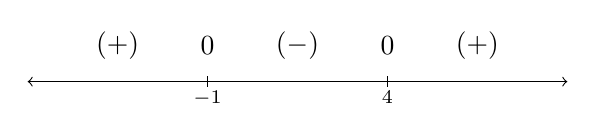
\begin{tikzpicture}
    \begin{axis}[axis equal image, ymin=-.15,ymax=.3,xmin=-1, xmax=2, axis x line=none, axis y line=none,]
	\draw[<->] (axis cs:-1, 0) -- (axis cs: 2, 0);
	\addplot[mark=|, only marks] coordinates {(0, 0)};
	\addplot[mark=|, only marks] coordinates {(1, 0)};
	\node[below] (z1) at (axis cs:0,0) {$\scriptstyle{-1}$};	
	\node[below] (z2) at (axis cs:1,0) {$\scriptstyle{4}$};
	\node (a) at (axis cs:-0.5,0.2) {$(+)$};
	\node (b) at (axis cs:1.5,0.2) {$(+)$};
	\node (c) at (axis cs:0.5,0.2) {$(-)$};	
	\node (d) at (axis cs:0,0.2) {$0$};	
	\node (e) at (axis cs:1,0.2) {$0$};	
    \end{axis}
\end{tikzpicture}
\end{image}

From the sign diagram, we see $r(x) \geq 0$ on $(-\infty, -1] \cup [4, \infty)$, which corresponds to where the graph of  $y=r(x) = 2^{x^2-3x} - 16$ is on or above the $x$-axis.

\end{explanation}

%\typeout{************************************************}
%\typeout{Dealing with Difficult Denominators}
%\typeout{************************************************}
\section{Dealing with Difficult Denominators}
Even after we feel comfortable with the procedure for solving inequalities involving continuous functions, you might still wonder about functions which aren't defined on all real numbers, such as rational functions or more generally, functions with denominators that could potentially evaluate to 0. The good news is that if $f$ and $g$ are continuous functions, the function $\frac{f}{g}$ is continuous wherever it is defined. Therefore, we can adapt our technique from before, but remembering that a change of sign \emph{could} happen around a point where a function is undefined, so we need to add any places our functions are undefined to our sign diagram.

\begin{example}
Solve the inequality $\dfrac{x^3-2x+1}{x-1} \geq \dfrac{1}{2}x-1$.
\end{example}
\begin{explanation}
To solve the inequality, it may be tempting to begin by clearing denominators. The problem is that, depending on $x$, $(x-1)$ may be positive (which doesn't affect the inequality) or $(x-1)$ could be negative (which would reverse the inequality).  Instead of working by cases, we collect all of the terms on one side of the inequality with $0$ on the other and begin to make a sign diagram.

\[ \begin{array}{rclr}

\dfrac{x^3-2x+1}{x-1} & \geq & \dfrac{1}{2}x-1 & \\ [10pt]

\dfrac{x^3-2x+1}{x-1}  - \dfrac{1}{2} x + 1& \geq & 0& \\ [10pt]

\dfrac{2\left(x^3-2x+1\right)-x(x-1)+1(2(x-1))}{2(x-1)} & \geq & 0 & \mbox{get a common denominator} \\ [10pt]

\dfrac{2x^3-x^2-x}{2x-2} & \geq & 0 & \mbox{expand} \\

\end{array} \]
Viewing the left hand side as a rational function $r(x)$ we make a sign diagram. The candidates for zeros of $r$ are the solutions to $2x^3-x^2-x=0$, which we can find by factoring. 
\begin{align*}
2x^3 - x^2 - x & = 0 \\
x(2x^2 - x - 1) & = 0\\
x(2x + 1)(x - 1) & = 0.
\end{align*}
Therefore, the candidates for zeros of $r$ are $x = 0$, $x = -\frac{1}{2}$ and $x = 1$. However, $x = 1$ is not in the domain of $r$, since it is the solution to $2x - 2 = 0$, which is the equation we get by setting the denominator equal to 0. However, $x$-values for which the function is undefined are also possible places where the sign of the function might change, so we should include them on the sign diagram. Since $r$ is a rational function, it is continuous everywhere it is defined, so when constructing the sign diagram, we only need to consider the intervals between zeros or places where it is undefined. For us, these intervals will be $\left(-\infty, -\frac{1}{2}\right)$, $\left(-\frac{1}{2}, 0\right)$, $(0, 1)$, and $(1, \infty)$. 

Choosing test values in each test interval (we encourage you to check the calculation), we can construct the sign diagram below. 
\begin{image}
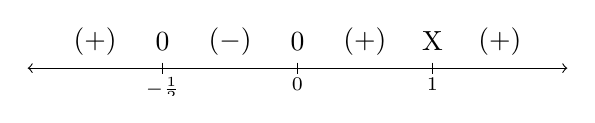
\begin{tikzpicture}
    \begin{axis}[axis equal image, ymin=-.2,ymax=.3,xmin=-1, xmax=3, axis y line=none, axis x line=none]
	\draw[<->] (axis cs:-1, 0) -- (axis cs: 3, 0);
	\addplot[mark=|, only marks] coordinates {(0, 0)};
	\addplot[mark=|, only marks] coordinates {(1, 0)};
	\addplot[mark=|, only marks] coordinates {(2, 0)};
	\node[below] (z1) at (axis cs:0,0) {$\scriptstyle{-\frac{1}{2}}$};
	\node[below] (z2) at (axis cs:1,0) {$\scriptstyle{0}$};
	\node[below] (z3) at (axis cs:2,0) {$\scriptstyle{1}$};
	\node (a) at (axis cs:-0.5,0.2) {$(+)$};
	\node (b) at (axis cs:1.5,0.2) {$(+)$};
	\node (c) at (axis cs:0.5,0.2) {$(-)$};	
	\node (d) at (axis cs:0,0.2) {$0$};	
	\node (e) at (axis cs:1,0.2) {$0$};	
	\node (f) at (axis cs:2, 0.2) {X};
	\node (g) at (axis cs: 2.5, 0.2) {$(+)$};
    \end{axis}
\end{tikzpicture}
\end{image}

We used an X to denote that $r$ is not defined at $x = 1$. 

We are interested in where $r(x) \geq 0$. We find $r(x)$ is positive on the intervals $\left(-\infty, -\frac{1}{2}\right)$, $(0,1)$ and $(1, \infty)$. We add to these intervals the zeros of $r$, $x = -\frac{1}{2}$, and $x = 0$, to get our final solution: $\left( - \infty, -\frac{1}{2} \right] \cup [0,1) \cup (1, \infty)$.

\end{explanation}

\begin{example}
Solve the inequality $\dfrac{e^x}{e^x - 4} \le 3$.
\end{example}
\begin{explanation}
The first step we need to take to solve  $\frac{e^{x}}{e^{x}-4} \leq 3$ is to get $0$ on one side of the inequality. To that end, we subtract $3$ from both sides and get a common denominator


\setlength{\extrarowheight}{12pt}
\[ \begin{array}{rclr}

\dfrac{e^{x}}{e^{x}-4} & \leq & 3 & \\

\dfrac{e^{x}}{e^{x}-4} - 3 & \leq & 0 & \\

\dfrac{e^{x}}{e^{x}-4} - \dfrac{3 \left(e^{x}-4\right)}{e^{x}-4} & \leq & 0 & \mbox{Common denomintors.} \\

\dfrac{12 - 2e^{x}}{e^{x}-4} & \leq & 0 & \\

\end{array}\]
\setlength{\extrarowheight}{2pt}

We set $r(x) = \frac{12 - 2e^{x}}{e^{x}-4}$. We note that $r$ is undefined when its denominator $e^{x}-4=0$, or when $e^{x} = 4$. Solving this by taking logarithms gives $x = \ln(4)$, so the domain of $r$ is $(-\infty, \ln(4)) \cup (\ln(4), \infty)$. To find the zeros of $r$, we set the numerator equal to zero and obtain $12 - 2e^{x} = 0$. Solving for $e^{x}$, we find $e^{x} = 6$, or $x = \ln(6)$. When we build our sign diagram, finding test values may be a little tricky since we need to check values around $\ln(4)$ and $\ln(6)$.  Recall that the function $\ln(x)$ is increasing\footnote{This is because the base of $\ln(x)$ is $e > 1$.  If the base $b$ were in the interval $0 < b < 1$, then $\log_{b}(x)$ would decreasing.} which means $\ln(3) < \ln(4) < \ln(5) < \ln(6) < \ln(7)$.  This indicates that we might want to use $\ln(3)$, $\ln(5)$, and $\ln(7)$ as our test values. While the prospect of determining the sign of $r\left(\ln(3)\right)$ may be very unsettling, remember that $e^{\ln(3)} = 3$, so \[r\left(\ln(3)\right) = \frac{12 - 2e^{\ln(3)}}{e^{\ln(3)}-4} = \frac{12-2(3)}{3-4} = -6\]  We determine the signs of $r\left(\ln(5)\right)$ and $r\left(\ln(7)\right)$ similarly and construct the sign diagram.

\begin{image}
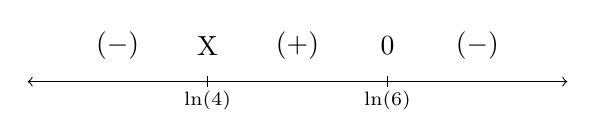
\begin{tikzpicture}
    \begin{axis}[axis equal image, ymin=-.15,ymax=.3,xmin=-1, xmax=2, axis x line=none, axis y line=none,]
	\draw[<->] (axis cs:-1, 0) -- (axis cs: 2, 0);
	\addplot[mark=|, only marks] coordinates {(0, 0)};
	\addplot[mark=|, only marks] coordinates {(1, 0)};
	\node[below] (z1) at (axis cs:0,0) {$\scriptstyle{\ln(4)}$};	
	\node[below] (z2) at (axis cs:1,0) {$\scriptstyle{\ln(6)}$};
	\node (a) at (axis cs:-0.5,0.2) {$(-)$};
	\node (b) at (axis cs:1.5,0.2) {$(-)$};
	\node (c) at (axis cs:0.5,0.2) {$(+)$};	
	\node (d) at (axis cs:0,0.2) {X};	
	\node (e) at (axis cs:1,0.2) {$0$};	
    \end{axis}
\end{tikzpicture}
\end{image}


From the sign diagram, we find our answer to be $(-\infty,\ln(4)) \cup [\ln(6), \infty)$.
\end{explanation}

\section{Conclusion}
We hope that the specific examples we've gone through illustrate a general principle when it comes to solving inequalities. First, we want to rewrite the inequality in a form where 0 is on one side and a nice-enough function is on the other side. Then, we use the fact that our functions are continuous on their domains to narrow down where possible sign changes can occur. From there, we can use test values to compute the sign of the function on intervals, and finish by putting our solution in interval notation. 

\end{document}
